\documentclass[12pt]{article}
\usepackage[utf8]{inputenc}
\usepackage{amsmath}
\usepackage{amssymb}
\usepackage{amsthm}
\usepackage{geometry}
\usepackage{pifont}
\usepackage{tikz}
\usetikzlibrary{automata, positioning, arrows}

\geometry{a4paper, margin=1in}

\title{Problem Set 3 - Solutions\\CPSC 326}
\author{Fernando, Dang, Raj, Eric M.}
\date{\today}

\begin{document}

\maketitle

\section*{Problem 1}

\textbf{Problem:} Consider the following Language:
$$L_1 = \{w \in \{a, b, c, d\}^* \mid |w|_a \geq |w|_c\}$$
Is $L_1$ a regular language? Prove your answer by either developing a DFA for $L_1$ or using the pumping lemma to show non-regularity.

\subsection*{Solution}

$L_1$ is \textbf{NOT regular}. We prove this using the pumping lemma.


Assume for contradiction that $L_1$ is regular. Let $p$ be the pumping length.

We can consider the string $w = c^p a^p \in L_1$ (since $|w|_a = p = |w|_c$, we have $|w|_a \geq |w|_c$).

We have $|w| = 2p \geq p$, so by the pumping lemma, we can write $w = w_1w_2w_3$ where:
\begin{enumerate}
    \item $|w_1w_2| \leq p$
    \item $|w_2| \geq 1$
    \item $w_1w_2^iw_3 \in L_1$ for all $i \geq 0$
\end{enumerate}

Since $|w_1w_2| \leq p$ and $w = c^p a^p$, the substring $w_1w_2$ consists entirely of $c$'s. Therefore, $w_2 = c^k$ for some $k \geq 1$.

Now we can consider $w_1w_2^2w_3 = c^{p+k}a^p$.

For this string: $|w_1w_2^2w_3|_a = p$ and $|w_1w_2^2w_3|_c = p + k$.

Since $k \geq 1$, we have $|w_1w_2^2w_3|_a = p < p + k = |w_1w_2^2w_3|_c$.

This means $|w_1w_2^2w_3|_a < |w_1w_2^2w_3|_c$, which violates the condition $|w|_a \geq |w|_c$.

Therefore, $w_1w_2^2w_3 \notin L_1$, which contradicts the pumping lemma.

Thus, $L_1$ is not regular.

\section*{Problem 2}

\textbf{Problem:} Consider the following Language:
\begin{align*}
L_2 = \{w \in \{0, 1, 2, 3, 4, 5, 6, 7, 8, 9\}^* \mid &\text{ the number of odd digits in } w\\
&\text{ equals the number of even digits in } w\}
\end{align*}
Is $L_2$ a regular language? Prove your answer by either developing a DFA for $L_2$ or using the pumping lemma to show non-regularity.

\subsection*{Solution}

$L_2$ is \textbf{NOT regular}. We prove this using the pumping lemma.


Assume $L_2$ is regular with pumping length $p$.

Consider the string $w = 0^p 1^p \in L_2$ (since it has $p$ even digits (all 0's) and $p$ odd digits (all 1's)).

We have $|w| = 2p \geq p$. By the pumping lemma, we can write $w = w_1w_2w_3$ where:
\begin{enumerate}
    \item $|w_1w_2| \leq p$
    \item $|w_2| > 0$
    \item $w_1w_2^iw_3 \in L_2$ for all $i \geq 0$
\end{enumerate}

Since $|w_1w_2| \leq p$ and $w = 0^p 1^p$, the substring $w_1w_2$ consists entirely of 0's. Therefore, $w_2 = 0^k$ for some $k > 0$.

Consider $w_1w_2^0w_3 = w_1w_3 = 0^{p-k}1^p$.

In this string:
\begin{itemize}
    \item Number of even digits = $p - k$
    \item Number of odd digits = $p$
\end{itemize}

Since $k > 0$, we have $p - k < p$, so the number of even digits does not equal the number of odd digits.

Therefore, $w_1w_3 \notin L_2$, which contradicts the pumping lemma.

Thus, $L_2$ is not regular.

\newpage

\section*{Problem 3}

\textbf{Problem:} Consider the following Language:
$$L_3 = \{w \in \{0, 1, \#\}^* \mid w = w_1\#w_2, w_1, w_2 \in \{0, 1\}^*, |w_1| + |w_2| \geq 3\}$$
Is $L_3$ a regular language? Prove your answer by either developing a DFA for $L_3$ or using the pumping lemma to show non-regularity.

\subsection*{Solution}

$L_3$ is a \textbf{regular language}. We can make a DFA with finitely many states.

\begin{center}
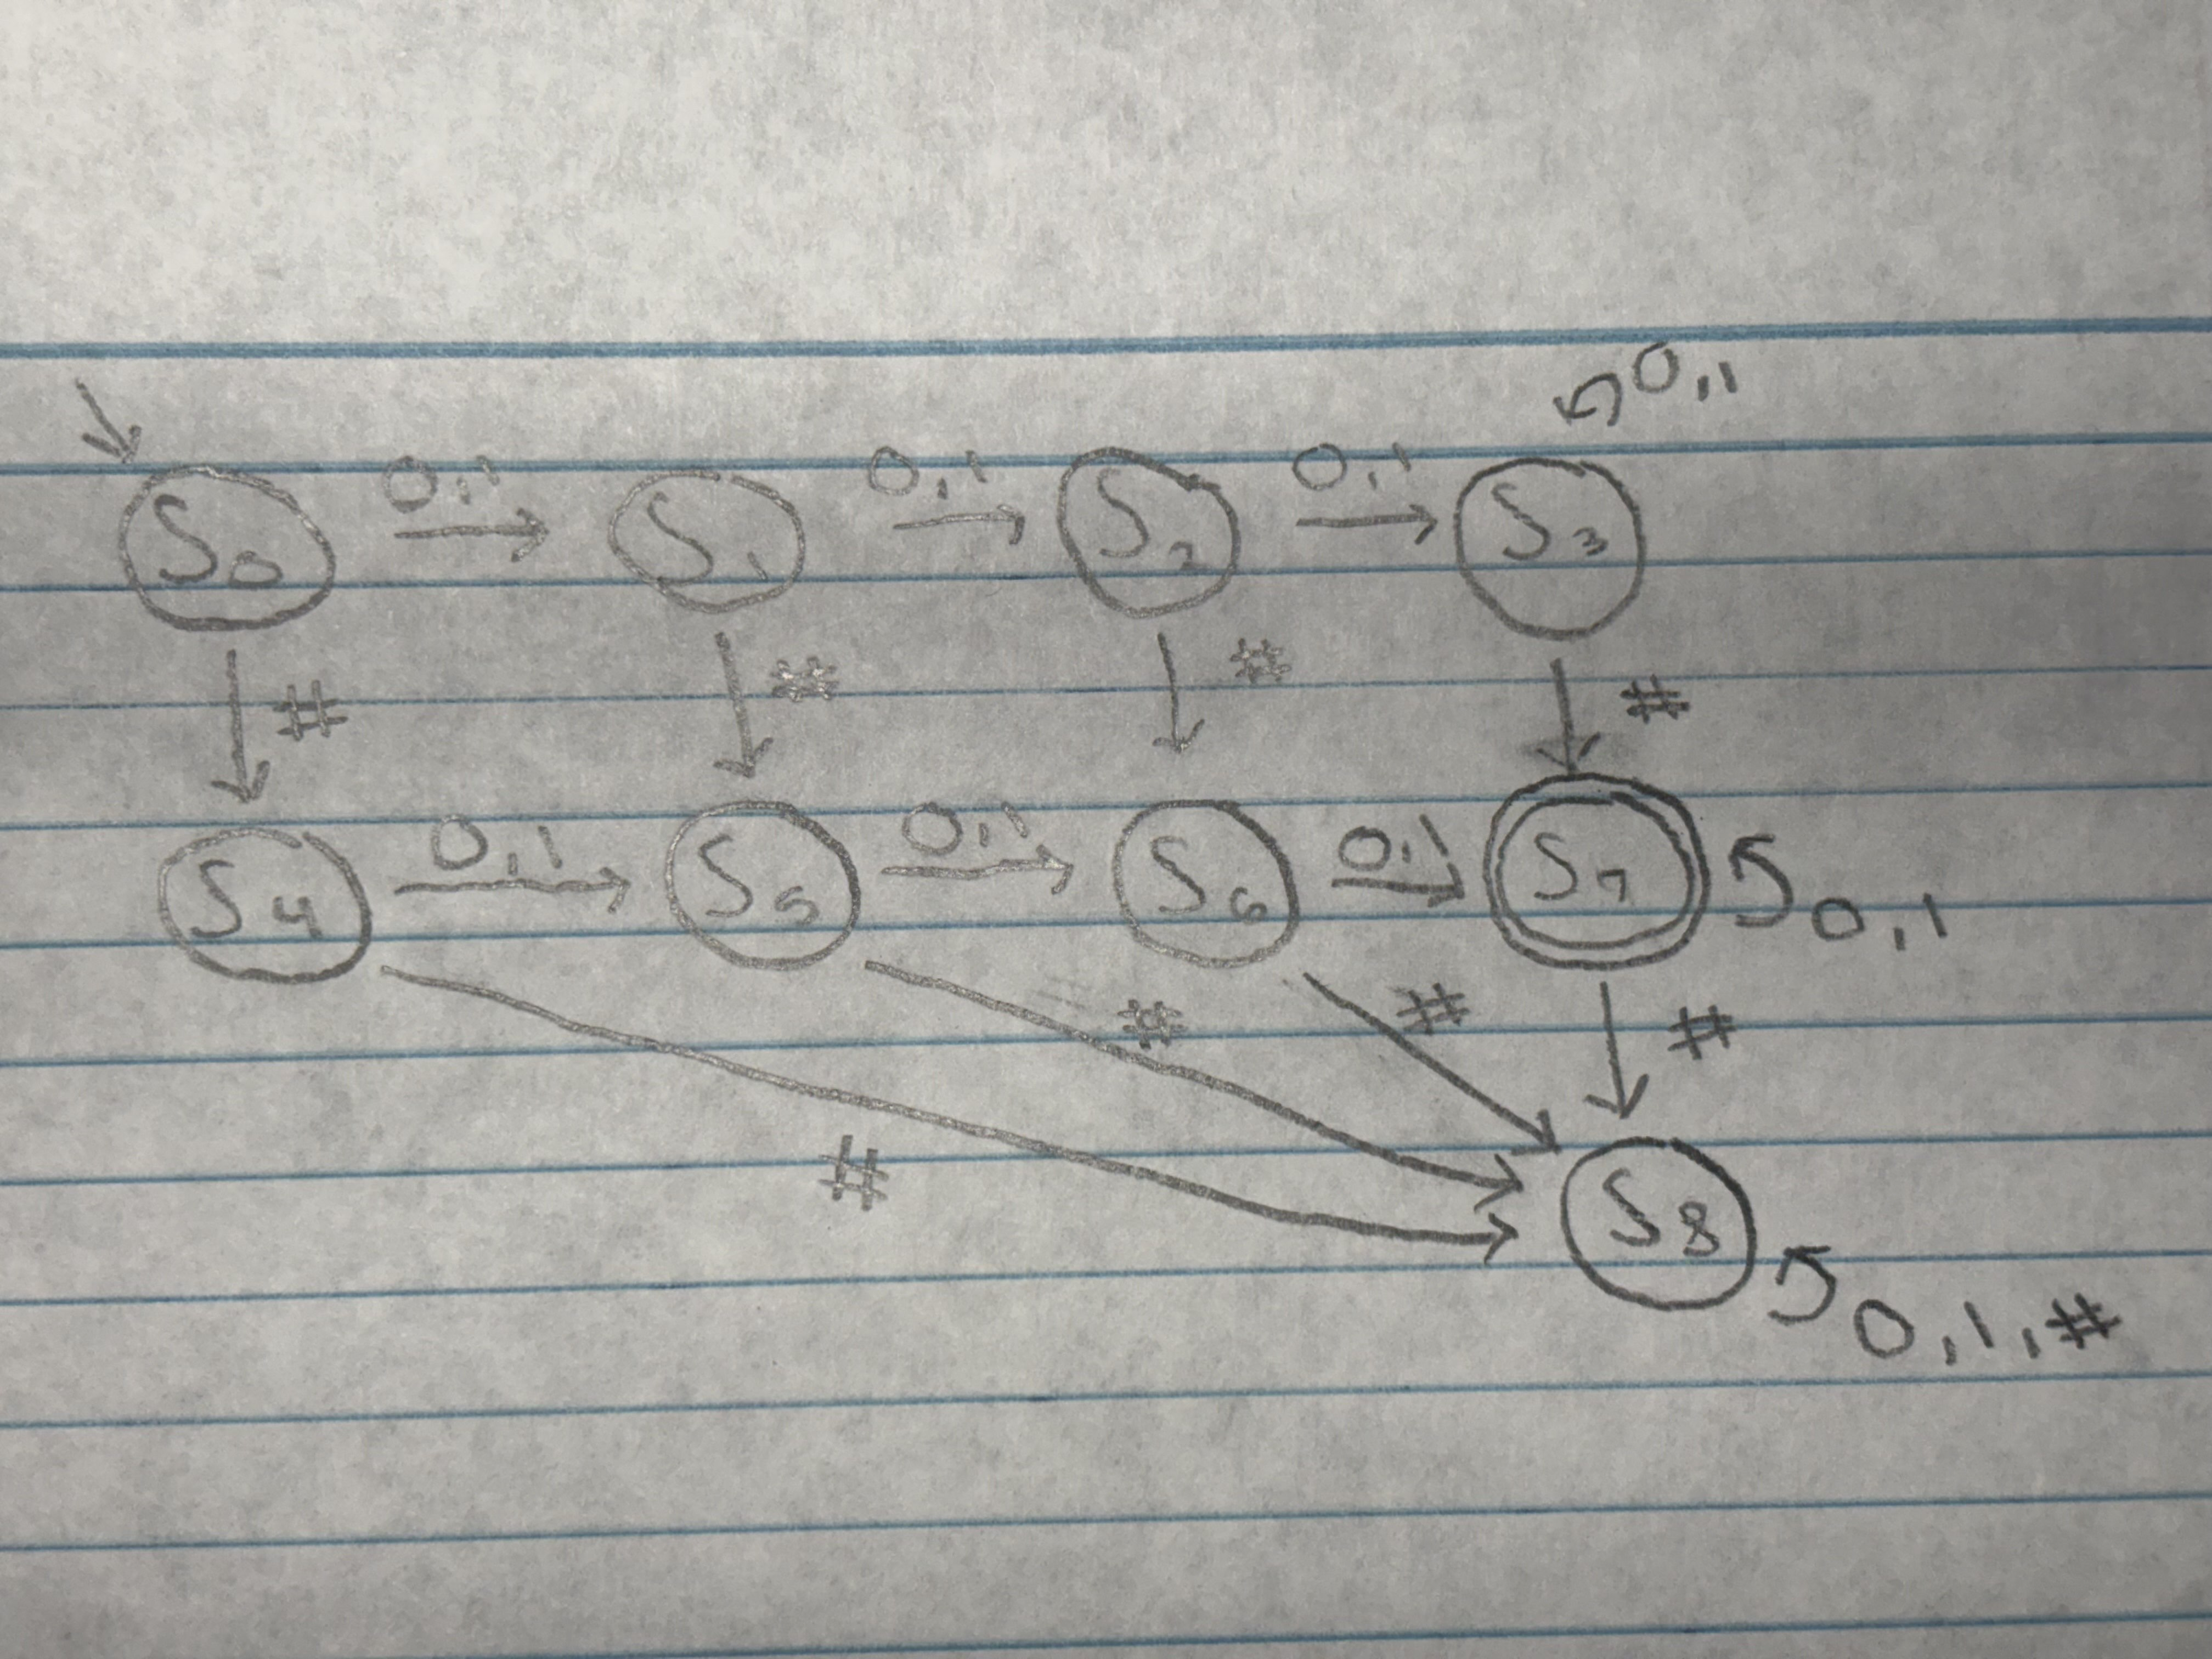
\includegraphics[width=0.8\textwidth]{problem3_diagram.png}
\end{center}




\newpage





\section*{Problem 4}

\textbf{Problem:} Design a DFA for the following regular language:
\begin{align*}
L_4 = \{w \in \{0, 1\}^* \mid &\text{if } |w|_0 \bmod 2 = 0, \text{ then } |w|_1 \bmod 3 = 0\\
&\text{ or if } |w|_0 \bmod 2 = 1 \text{ then } |w|_1 \bmod 2 = 0\}
\end{align*}

\subsection*{Solution}


\begin{center}
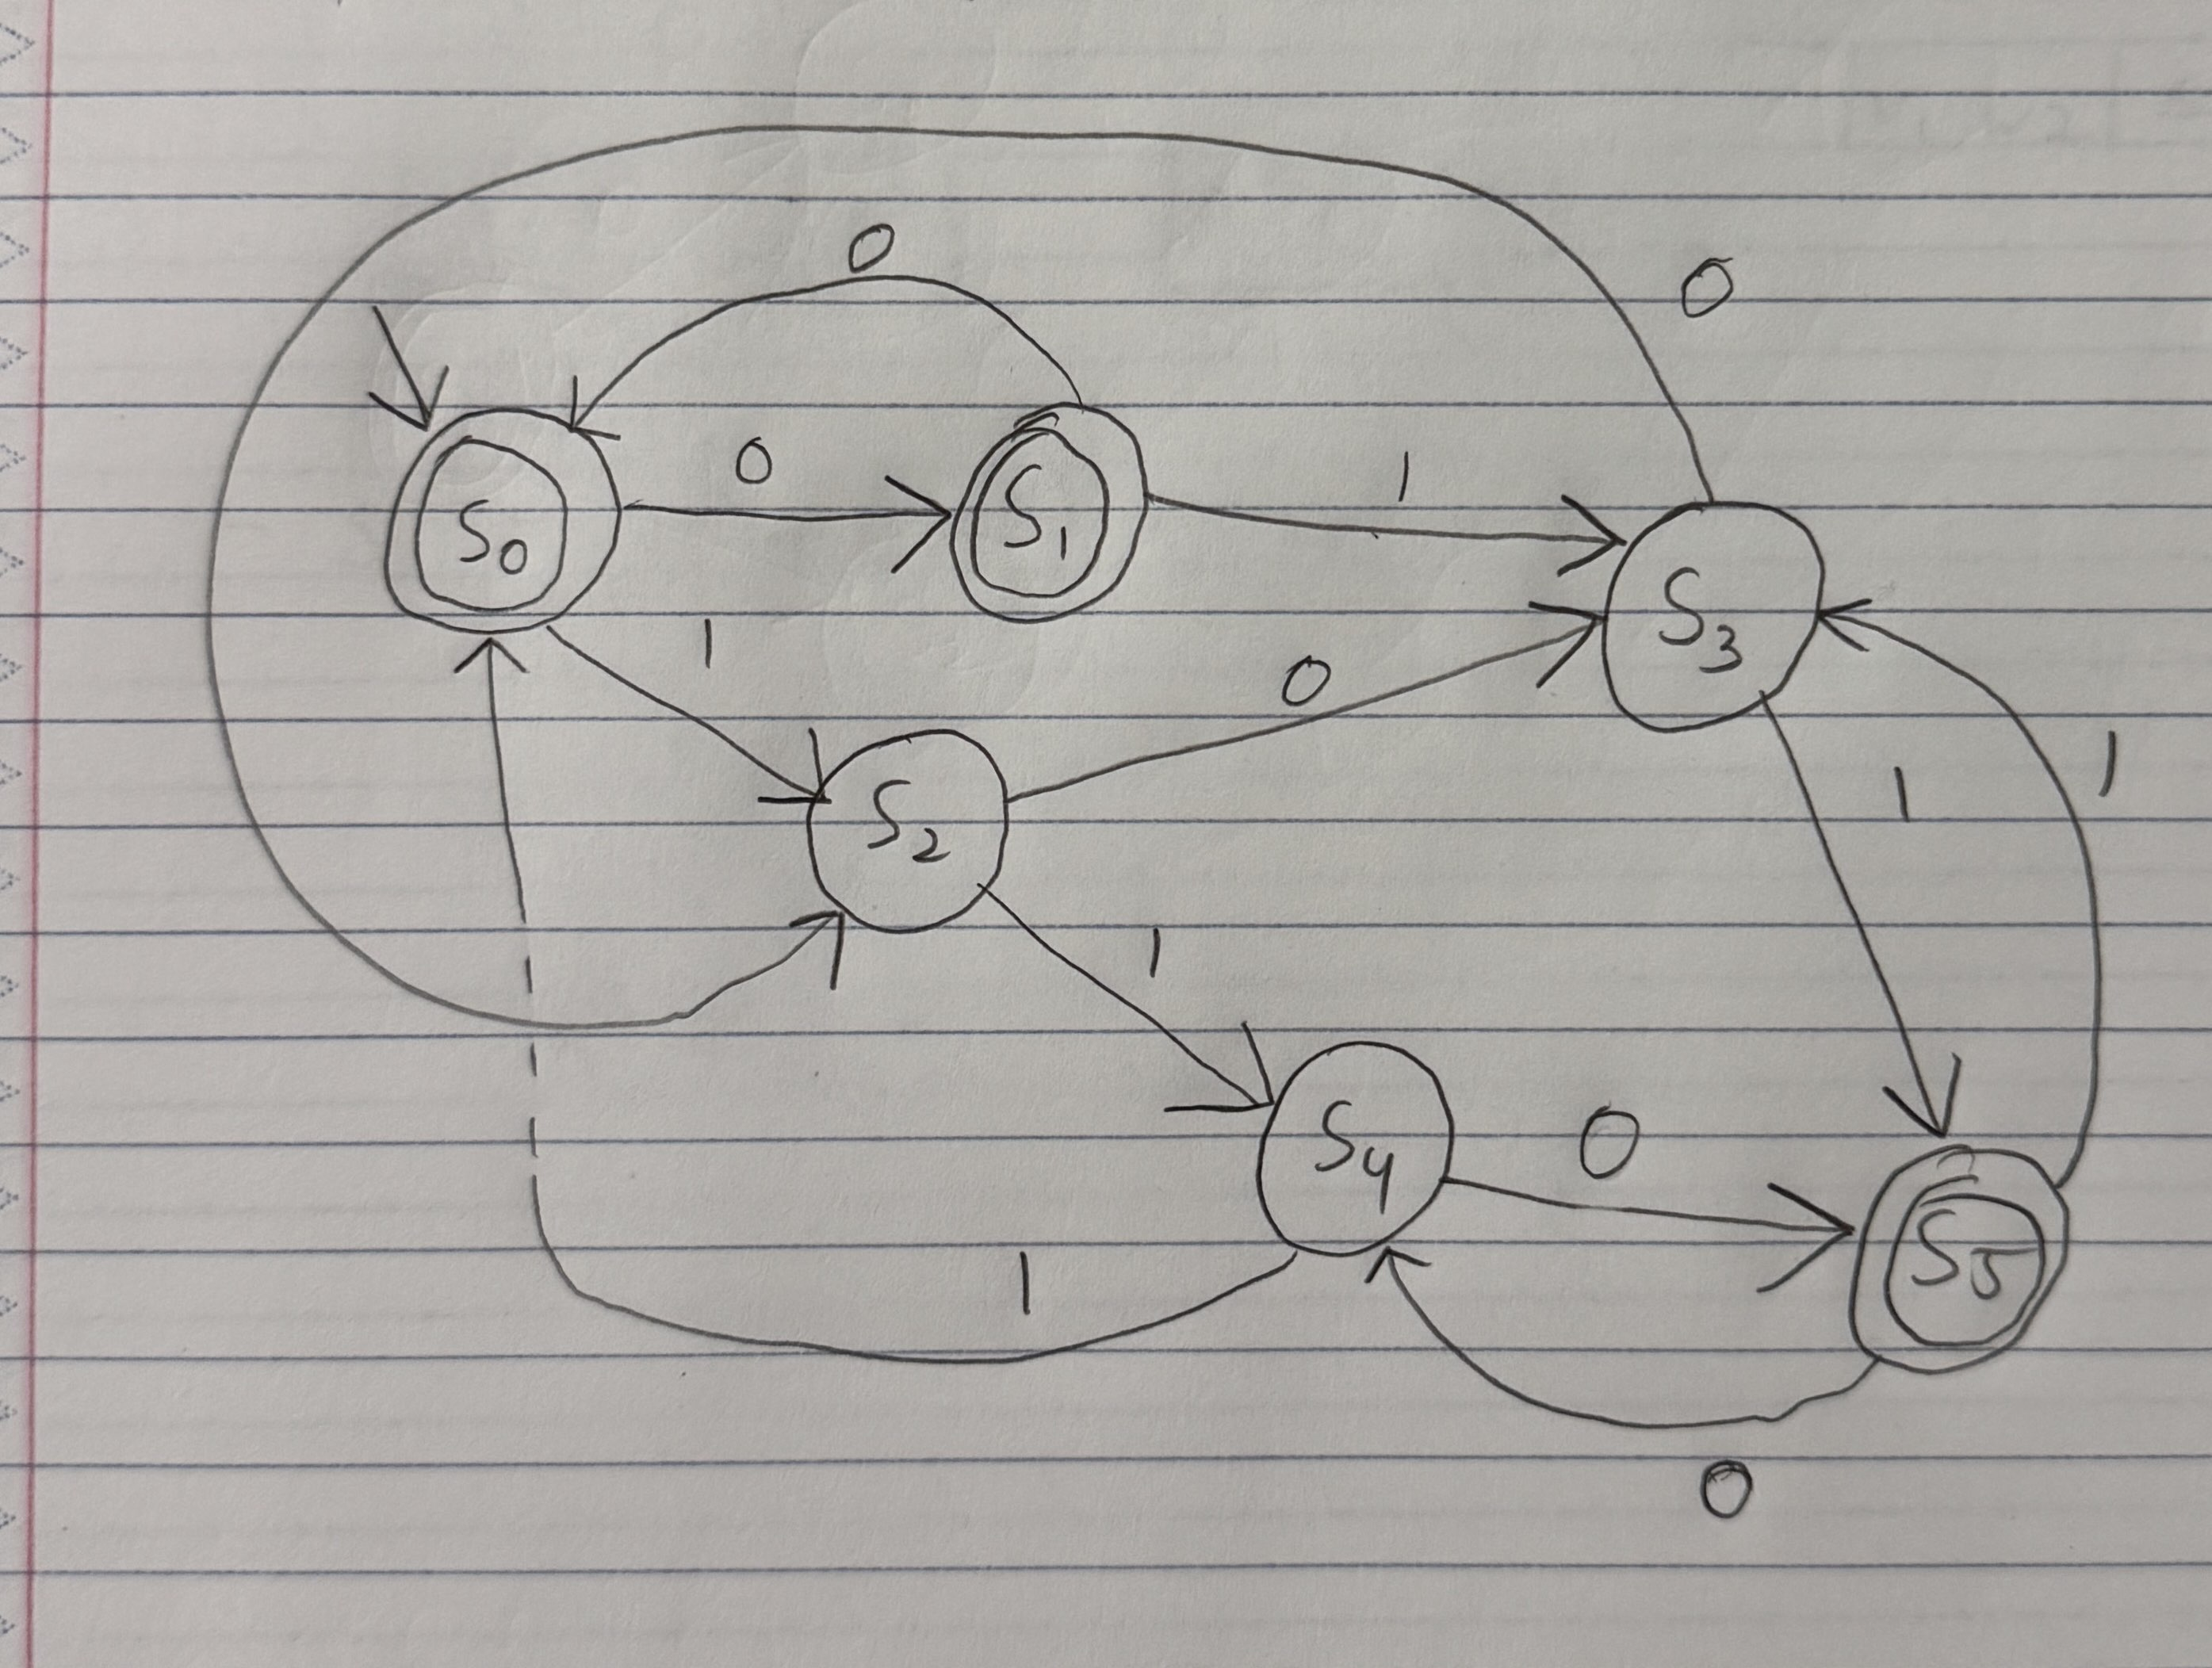
\includegraphics[width=0.9\textwidth]{problem4_diagram.png}
\end{center}

\end{document}